% !TeX program = xelatex

\chapter{Anforderungsanalyse der Software}

\section{Rückblick auf die originale Anwendung}
Um die Anforderungen an die neue und erweiterte Software zu verstehen, bietet es sich an ersteinmal sich den Ausgagspunkt der originalen Software anzuschauen.
Diese wurde als \acf{SPA} entwickelt. Sie besaß eine recht flache hierarchie und bildete die Datenstruktur des Backends ab. Das bedeutet, dass der Nutzer anstatt in verschiedenen Untermenüs zu navigieren, nur tiefer in die Beschreibung des \textit{Projects} eintaucht.
Dieses Vorgehen stellte sich al eine intuitive Lösung für den Nutzer heraus.


Zu beginn bekam der Nutzer direkt auf der Hauptseite eine Übersicht über alle \textit{Projects}, die er angelegt hat und die Möglichkeit neue Projekte anzulegen, zu bearbeiten, zu löschen oder hochzuladen (siehe Abbildung \ref{fig:old_mainpage_start}).
Ein Nutzeraccount an sich gab es nicht. Somit teilten sich alle Nutzer im Netzwerk die gleichen \textit{Projects}.

\begin{figure}[htbp]
    \centering
    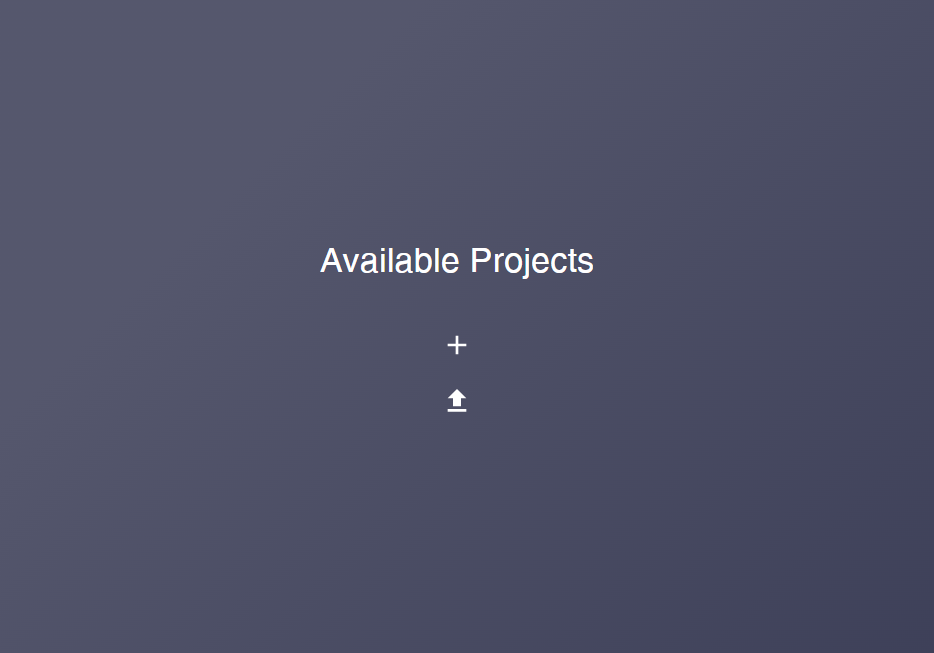
\includegraphics[width=0.9\linewidth]{includes/figures/old_version/ui_old_mainpage.png}
    \caption{Hauptansicht der originalen Anwendung, hier sind alle Projekte aufgelistet}
    \label{fig:old_mainpage_start}
\end{figure}

Um seine \textit{Projects} zu bearbeiten, muss der Nutzer auf den entsprechenden Button klicken und wird auf die Projektseite weitergeleitet. Dort findet sich eine Übersicht über alle vorhandenen \textit{Tracks}, 
Optionen diese zu bearbeiten und neue \textit{Tracks} anlegen. Auch finden sich innerhalb des \textit{Tracks} die einzelnen \textit{DataSets}, welche frei erstellt, bearbeitet, verschoben und gelöscht werden können (siehe Abbildung \ref{fig:dataset_old_version}).
Dies spiegelt die originale Datenstruktur wieder. Ein \textit{Project} besteht aus mehreren \textit{Tracks}, welche wiederum aus mehreren \textit{DataSets} bestehen. Die Abfolge wurde gewählt, damit Nutzer mehrere \textit{Track} parallel senden, 
und über die sukzessiv abgearbeiteten \textit{DataSets} die Struktur des im jeweiligen \textit{Tracks} definieren können.

\begin{figure}[htbp]
    \centering
    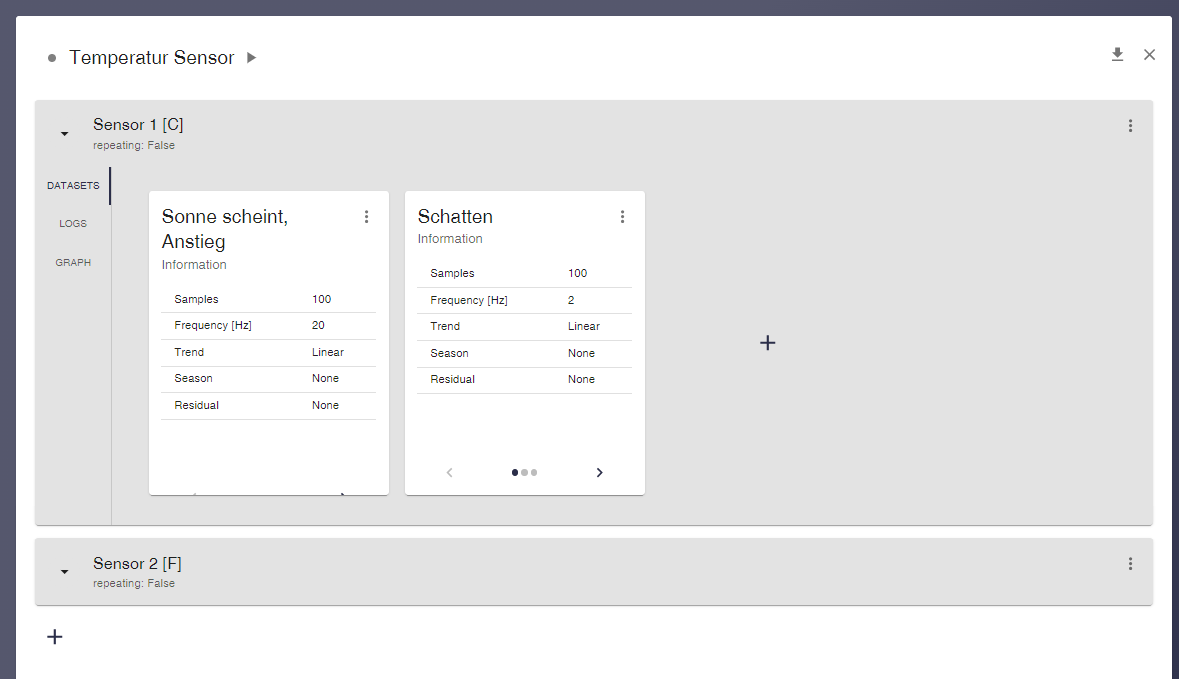
\includegraphics[width=0.9\linewidth]{includes/figures/old_version/ui_old_dataset.png}
    \caption{\textit{DataSet} Ansicht der originalen Anwendung}
    \label{fig:dataset_old_version}
\end{figure}

Das Senden der Daten erfolgt über einen entsprechenden Button, welcher, während gesendet wird, entsprechend der Abbildung \ref{fig:dataset_old_sending} innerhalb der \textit{Projects}-Seite und der Übersicht rot leuchtet und somit den Sendevorgang auch visuell bestätigt.

\begin{figure}[htbp]
    \centering
    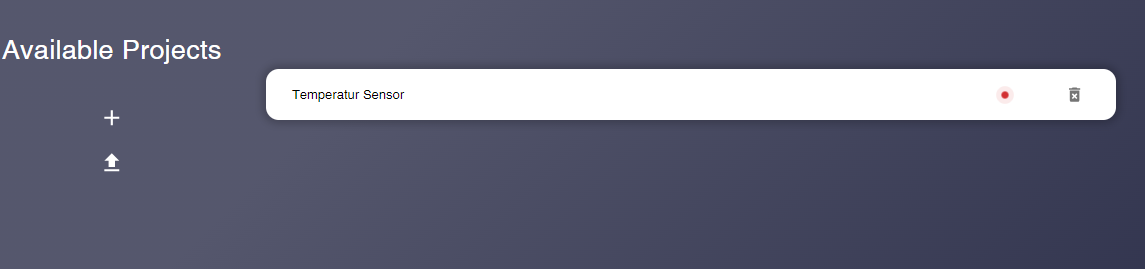
\includegraphics[width=0.9\linewidth]{includes/figures/old_version/ui_old_projects.png}
    \caption{\textit{DataSet} Ansicht der originalen Anwendung}
    \label{fig:dataset_old_sending}
\end{figure}

Themen wie Eingabenvalidierung und Fehlerbehandlung wurden in der originalen Version nur durch JsonSchema vorgenommen und nicht tiefer konzeptioniert.
Flexibilität der zu sendenden Datentypen gab es auch nicht. Aufbauend auf dem gegebenen Schema wurden Fließkommazahlen generiert und versendet.
Auch wurde angenommen, dass der Nutzer der englischen Sprache mächtig ist und die Eingabeanforderungen und Beschreibungen versteht.





\label{cha:Anforderungsanalyse}
Eine Software, welche sowohl Daten generieren, als auch anhand von Daten trainieren soll kommt mit einer vielzahl an Anforderungen.
Grundsätzlich ist Datengenerierung bereits komplexes Thema, aber hierfür wurde im Ursprünglichen Projekt bereits ein Konzept erstellt. Dieses muss nur um neue Funktionalität erweitert/vorhandene Konzepte angepasst werden.
Trainieren anhand von Daten benötigt aber ein eigenes Konzept. Um beide Systeme zusammenzuführen, muss grob auf 5 Punkte geachtet werden.

\begin{itemize}
    \item Datenmanagement
    \item Trainieren der Modelle
    \item Benutzerschnittstelle und Benutzererfahrung
    \item Sicherheit und Privatsphäre
    \item Technische Anforderungen
\end{itemize}

Neben diesen 4 Punkten müssen auch ein paar technische Anforderungen erfüllt werden.


\section{Anforderungen an die Software}
\subsection{Datenmanagement}
\label{cha:Anforderungsanalyse:Datenmanagement}
Ein großer und elementarer Teil der zu erstellenden Software wird es sein, Daten zu verwalten und in verschiedensten Elementen der Software zu verarbeiten. Hierfür bedarf es eines sinnvollen Konzepts, 
um die Anforderungen der Software formulieren zu können.

Das spätere System muss in der Lage sein, Daten aus unterschiedlichen Quellen mit verschiedenen Datenformaten effizient zu verarbeiten. Da es Ziel ist, Daten aus fremden Quellen im System zu verarbeiten, 
müssen vom System gängige Formate verarbeitet werden. Eine solche Flexibilität ermöglicht dem System eine einfache Benutzung und eine breite Anwendbarkeit in verschiedenen Szenarien und erleichtert dem Nutzer die Handhabung der Software. Für die Verarbeitung verschiedener Datenformate muss eine universelle Verarbeitungslogik 
entwickelt werden, die diese in ein für das System nutzbares Format konvertiert und, da Formate wie JSON und CSV flexibel sind, diese auf valide Inhalte überprüft. Effizienter Umgang mit großen Datenmengen ist ebenfalls wichtig, 
um die Ressourcen schwächerer Systeme nicht zu überlasten. Entsprechende Vorverarbeitungsschritte müssen vom System durchgeführt werden. Die Umsetzung dieser Funktionen erfordert ein visuelles Bestätigungswerkzeug, das die Auswirkungen der 
Datenmanipulation in Echtzeit anzeigt und so eine transparente und zugängliche Benutzererfahrung schafft. Zudem muss sichergestellt werden, dass ausgewählte Vorverarbeitungsschritte reversibel sind, sodass Nutzer die Möglichkeit haben, die 
Vorverarbeitung und ihre spezifischen Parameter zu speichern und zu einem späteren Zeitpunkt zu nutzen oder zu verändern.

Das gesamte Konzept des Datenmanagements muss zudem erweiterbar sein, um neue Funktionalitäten und Abhängigkeiten in Zukunft zu ermöglichen. Das Datenmodell muss daher Möglichkeiten bieten, um neue Datenformate und Vorverarbeitungsschritte zu 
integrieren. Während dies die Komplexität und den initialen Aufwand erhöht, wird es die Wartung und Erweiterung der Software in Zukunft erleichtern.


\subsection{Trainieren und Konfigurieren von Modellen}
\label{concept:training}
In der Anforderungsanalyse für das Training von \ac{ML} Modellen sowie Zeitreihenzerlegungs- und Analysealgorithmen liegt der Fokus auf der Entwicklung einer benutzerfreundlichen, effizienten und interaktiven Trainingsumgebung.
Da es nicht möglich ist, den richtigen Algorithmus für alle Anwendungsfälle zu finden, muss die Software eine Vielzahl von Algorithmen bereitstellen, die jeweils detailliert in Bezug auf ihre Eigenschaften und Anwendungsbereiche beschrieben werden.
Wesentlich ist hierbei eine intuitive Konfiguration aller Algorithmen, die auch für Benutzer ohne spezialisiertes Wissen in diesen Bereichen zugänglich ist. 
Gleichzeitig sollte eine Balance zwischen einfacher Bedienbarkeit und der Möglichkeit zur Feinabstimmung der Modelle gefunden werden, um eine breite Nutzerbasis zu bedienen.

Da das Training von Modellen eine rechenintensive Aufgabe darstellt, muss die Software eine effiziente Nutzung der Systemressourcen sicherstellen, um auch auf weniger leistungsfähigen Systemen eine reibungslose Funktion zu garantieren.
Dies ist wichtig, da die Infrastruktur der Software nicht nur auf leistungsstarken Servern, sondern auch auf lokalen Systemen mit begrenzten Ressourcen betrieben werden soll.

Abschließend ist die transparente Darstellung der Trainings- und Validierungsergebnisse entscheidend. Die Ergebnisse sollten schnell und effizient präsentiert werden und sich an unterschiedliche Benutzeranforderungen anpassen lassen. 
Dies gewährleistet, dass die Trainingskomponente der Software sowohl für Experten als auch für Laien geeignet ist, was die Zugänglichkeit und Effektivität der Software insgesamt steigert.


\subsection{Benutzerschnittstelle und Benutzererfahrung}
\label{cha:Anforderungsanalyse:Usability}

Die Gestaltung der Benutzeroberfläche der Software erfordert ein tiefgreifendes Verständnis für die Bedürfnisse und Erwartungen der Nutzer. 
Der Nutzer muss im Zentrum aller Designentscheidungen stehen, wobei das Ziel ist, eine Umgebung zu schaffen, in der sich die Benutzer sicher und kompetent in ihren Interaktionen fühlen und stets die Kontrolle über die Software behalten. 
Um dies zu erreichen, ist eine effiziente und benutzerfreundliche Oberfläche unerlässlich.

Gemäß der ISO 9241-110\footnote{Die ISO Norm 9241-110, auch als Grundsätze der Dialoggestaltung bekannt, behandelt die ergonomische Gestaltung von interaktiven Systemen und unterteilt diese in sieben Grundkonzepte.} lassen sich 
verschiedene grundlegende Anforderungen identifizieren, die für die Gestaltung einer effektiven Benutzeroberfläche wesentlich sind. Nachfolgend werden diese Anforderungen, basierend auf der Interpretation aus \cite{DieGrund14:online}, dargestellt:

\begin{description}
    \item[Aufgabenangemessenheit] Die Benutzeroberfläche sollte so gestaltet sein, dass Voreinstellungen von Standardwerten und die Struktur der Dialogwege die Aufgaben des Benutzers widerspiegeln und unterstützen.
    \item[Steuerbarkeit] Die Benutzer müssen die Möglichkeit haben, die Abfolge und Tiefe der angebotenen Dialoge nach ihren Bedürfnissen zu steuern.
    \item[Erwartungskonformität] Alle Aktionen und Steuerelemente in der Software sollten nachvollziehbar und konsistent mit den Erwartungen des Benutzers sein.
    \item[Selbstbeschreibungsfähigkeit] Die Software sollte Wartezeiten visualisieren, klare Links bereitstellen und bei Bedarf Hilfestellungen anbieten, um dem Benutzer stets Orientierung zu geben.
    \item[Lernförderlichkeit] Die Software sollte eine klare, logische und sinnvolle Strukturierung komplexer Aufgaben bieten, um eine einfache Erlernbarkeit zu gewährleisten.
    \item[Fehlertoleranz] Eingabefehler sollten angemessen behandelt werden, ohne dass die Software abstürzt, und der Benutzer sollte weiterhin in der Lage sein, seine Ziele zu erreichen.
    \item[Individualisierbarkeit] Die Software sollte es dem Benutzer ermöglichen, die Oberfläche und Funktionalitäten an seine individuellen Bedürfnisse anzupassen.
\end{description}

Eine weitere wichtige Anforderung ist die Bereitstellung von mehrsprachigkeit. Software, gerade wenn sie komplexe Themen aufgreift, sollte die mentale Leistung seiner Nutzer nicht unnötig belasten, indem man Fachthemen in einer Fremdsprache behandelt.
Dies kann zu Missverständnissen und Fehlern führen, die die Effektivität der Software beeinträchtigen. 
Die Berücksichtigung dieser Prinzipien stellt sicher, dass die Benutzeroberfläche nicht nur funktional und effizient ist, sondern auch ein angenehmes und effektives Benutzererlebnis bietet, 
das auf die Bedürfnisse und Fähigkeiten verschiedener Nutzergruppen zugeschnitten ist.




\subsection{Sicherheit und Privatsphäre}
Da es ein integraler Teil der Software sein wird, eigene Daten hochzuladen, diese zu speichern und zu verarbeiten, ist die Anforderung an einen vernünftigen Datenschutz und Datensicherheit notwendig. 
Um den Schutz dieser sensiblen Benutzerdaten zu gewährleisten, ergeben sich aus den folgenden rechtlichen Rahmenbedingungen spezifische Anforderungen.

Unter Berücksichtigung der EU-Datenschutz-Grundverordnung (DSGVO) müssen technische und organisatorische Maßnahmen implementiert werden, um ein angemessenes Schutzniveau für die 
Verarbeitung personenbezogener Daten sicherzustellen. Insbesondere Artikel 32 DSGVO fordert die Verschlüsselung und sichere Verarbeitung von Daten, um sie vor unbefugtem Zugriff zu schützen. Dies beinhaltet in diesem Fall auch den 
Schutz vor anderen Nutzern. Während die hochgeladenen Daten nicht zwangsläufig die Identifikation einer Person ermöglichen, können sie dennoch Daten enthalten, welche Rückschlüsse auf eine Person zulassen könnten. 
Beispielsweise können Sensordaten der Haussteuerung Rückschlüsse auf die Gewohnheiten und das Verhalten einer Person zulassen. Dies muss durch entsprechende Maßnahmen abgesichert werden. Hieraus ergibt sich aber auch eine technische Anforderung. 
Da es sich bei der Anwendung um eine Webanwendung handelt, müssen die gesamten Strukturen, die ein Nutzer pflegt, separiert werden. Hierfür ist ein entsprechendes Konzept zu entwickeln.

Zusammenfassend ist es von höchster Wichtigkeit, dass die Anwendung ein robustes Sicherheitssystem implementiert, welches den rechtlichen Anforderungen entsprechend die Privatsphäre sowie die Sicherheit der Benutzerdaten effektiv schützt.


\subsection{Technische Anforderung}
Da sich in eine Vielzahl von Komponenten in der Entwicklung der Software abzeichnet, ist eine präzise und effektive Kommunikation zwischen diesen Komponenten unerlässlich, 
um die Gesamtfunktionalität der Anwendung zu gewährleisten. Daher sind umfassende Dokumentationen für jede Komponente entscheidend. Diese sollten nicht nur die Funktionsweise der einzelnen Komponenten detailliert beschreiben, sondern 
auch die Kommunikationsprotokolle und Schnittstellen zwischen ihnen klar darlegen. Eine solche Dokumentation ermöglicht die entwicklung der Systemarchitektur vollständig zu verstehen und effizient damit zu arbeiten.

Ein weiterer wichtiger Aspekt ist die einheitliche Fehlerbehandlung über die APIs. Ein konsistenter Ansatz in diesem Bereich erleichtert es dem Frontend, Fehler schnell zu identifizieren, zu verarbeiten und in einer für die Nutzer 
verständlichen Weise zu kommunizieren. Diese Konsistenz in der Fehlerbehandlung ist entscheidend für die Benutzerfreundlichkeit und die Stabilität der Anwendung.

Zusätzlich ist die Implementierung von Überwachungssystemen von großer Bedeutung, um den Zustand der Anwendung kontinuierlich zu überprüfen und mögliche Probleme frühzeitig zu erkennen. Solche Systeme sollten in der Lage sein, schnell 
auf erkannte Fehler zu reagieren und geeignete Maßnahmen zur Fehlerbehebung einzuleiten oder entsprechende Stellen darüber zu informieren.

Abschließend spielt auch die Einfachheit des Deployments eine wesentliche Rolle. Die Bereitstellung und Inbetriebnahme der Anwendung sollte so unkompliziert wie möglich sein, um eine effiziente und reibungslose in Betriebnahme zu 
gewährleisten. Dies umfasst sowohl die Erstinstallation als auch die Durchführung fortlaufender Updates. Durch die Berücksichtigung dieser 
Anforderungen wird sichergestellt, dass die Software nicht nur ihre Kernfunktionen erfüllt, sondern auch hohe Nutzerzufriedenheit und geringe Wartungsaufwände bietet.



\subsection{Anforderungen an die Software}
Fässt man die in den vorherigen Kapitel gesammelten Anforderungen zusammen, ergibt sich folgende Liste an Anforderungen an die Software:
\begin{enumerate}
    \item \textbf{Vielseitige Datenintegration und Unterstützung mehrerer Datenformate:} Unterstützt verschiedene Datenquellen und Formate, um eine flexible Datenhandhabung zu gewährleisten.
    \item \textbf{Effiziente Datenübertragung, -validierung und Systemressourcennutzung:} Sorgt für schnelle und korrekte Datenverarbeitung sowie optimale Nutzung der Systemressourcen.
    \item \textbf{Benutzerorientierte Datenauswahl und -vorverarbeitung sowie Verwaltung:} Ermöglicht es Nutzern, Daten auszuwählen und vorzubereiten, einschließlich Qualitätsoptimierung und reversibler Vorverarbeitungsschritte.
    \item \textbf{Visuelles Feedback, Datenexploration und transparente Ergebnisdarstellung:} Bietet klare visuelle Darstellungen und Werkzeuge zur Datenexploration, um Benutzern das Verständnis der Daten und Ergebnisse zu erleichtern.
    \item \textbf{Sicherheit, Privatsphäre und sicherer Umgang mit Benutzerdaten:} Gewährleistet Datenschutz und sichere Datenverarbeitung, einschließlich Zugriffskontrollen und Datentrennung.
    \item \textbf{Trainieren der Modelle und Bereitstellung einer Vielzahl von Algorithmen:} Ermöglicht das Trainieren verschiedener Modelle und bietet eine breite Palette an Algorithmen mit Beschreibungen und Anwendungsbereichen.
    \item \textbf{Benutzerschnittstelle, Benutzererfahrung und intuitive Konfiguration der Algorithmen:} Stellt eine benutzerfreundliche Oberfläche und einfache Konfigurationsmöglichkeiten der Algorithmen bereit.
    \item \textbf{Dokumentation, Fehlerbehandlung, Überwachung und Deployment:} Umfasst eine umfassende Dokumentation, einen einheitlichen Ansatz zur Fehlerbehandlung, Überwachung der Anwendungsperformance und vereinfachtes Deployment.
\label{list:requirements}
\end{enumerate}

Auf grundlage der hier definierten Anforderungen lässt sich direkt eine grobe Struktur des Projektes ableiten, unabhängig von den genutzten Technologien. Dieses wird im folgenden Abschnitt erläutert.
Die gewählten Technologien und deren Umsetzung wird in den Kapiteln \ref{cha:Implementation} und \ref{cha:setup} erläutert.





\section{Konzeption der Software}
\subsection{Datenmanagementkonzept}
Um die Anforderungen an das Datenmanagement zu erfüllen, muss ein Konzept entwickelt werden, das die Integration, Validierung und Verarbeitung von Daten ermöglicht. Da das System eine Vielzahl an Daten und Formaten unterstützen soll, 
ist die Entwicklung einer Datenstruktur sinnvoll, die alle Formate abbilden kann. Eine geeignete Lösung wäre die Konvertierung der Originaldaten in ein systemkompatibles Array-Format, wie beispielsweise Listen, die in den meisten 
Programmiersprachen einfach und effizient verarbeitet werden können.

Da es sich um Dokumente handelt, ist eine angemessene Persistenzmethode erforderlich. Um dies mit der relationalen Struktur des ursprünglichen Projekts zu verbinden, bietet sich eine Separation oder Kombination an. PostgreSQL, eine relationale Datenbank, 
die JSON-Dokumente speichern kann, wäre hierfür eine geeignete Wahl. Formate wie JavaScript Object Notation (JSON), Comma Separated Values (CSV) oder binäre Array-Formate wie NumPy-Arrays unterstützen solche Strukturen. Werden diese durch eine universelle 
Verarbeitungslogik in ein nutzbares Format konvertiert, muss die Validierung dem Nutzer aussagekräftiges Feedback zu möglichen Fehlern geben.

Im Rahmen der Vorverarbeitung muss es Nutzern möglich sein, hochgeladene Daten durch eine Reihe von Transformationsschritten zu leiten, die zur Optimierung der Datenqualität und zur 
Erleichterung des Lernprozesses der Algorithmen unerlässlich sind. Zu diesen Schritten gehören die Normalisierung der Daten, um eine einheitliche Skala zu erreichen, die optionale Entfernung linearer Trends zur 
Hervorhebung stationärer Komponenten in Zeitreihen und die frei wählbare Reduktion des Datenvolumens durch gezielte Verfahren. Bei mit Zeitstempeln versehenen Daten müssen eventuelle Lücken adäquat behandelt werden.

Angesichts der Komplexität dieser Schritte ist es wichtig, dass Nutzer Rückmeldungen zu ihren Änderungen oder Konfigurationen erhalten. Visualisierungswerkzeuge wie dynamische Graphen oder interaktive 
Datenexplorationsschnittstellen spielen dabei eine Schlüsselrolle. Sie ermöglichen es Nutzern, komplexe Datentransformationsprozesse zu visualisieren und deren Einfluss auf die 
resultierenden Daten und deren Qualität zu verstehen. Werden die Konfigurationen getrennt von den Originaldaten gespeichert, stellt die Reversibilität der Aktionen kein Problem dar.

Neben den Trainingsdaten müssen auch andere Datenstrukturen erstellt werden, die alle Notwendigkeiten rund um die neuen und alten API-Bereiche abdecken, da das bestehende Datenmodell nicht in der Lage ist, 
diese neuen Abhängigkeiten abzubilden. Ziel des Datenmanagementmoduls ist es, eine robuste, nutzerzentrierte Plattform für die Datenaufbereitung zu schaffen, die den Weg für präzises und effektives maschinelles Lernen ebnet.


\subsection{Konzeption des Modelltrainings}
Wie in der Sektion \ref{concept:training} erörtert, müssen verschiedene Algorithmen mit spezifischen Eigenschaften und Fähigkeiten zur Verfügung gestellt werden. Die Benutzeroberfläche der Webanwendung muss daher eine Auflistung dieser Algorithmen bereitstellen, 
inklusive einer detaillierten Beschreibung ihrer Anwendungsbereiche und Leistungsmerkmale, um Benutzern eine informierte Auswahl zu ermöglichen, die ihren spezifischen Anforderungen und dem Kontext ihrer Daten gerecht wird.
Da sich die Software nicht nur an Informatiker richtet, ist dies extrem wichtig.

Die individuelle Konfiguration der Modelle stellt eine Herausforderung dar, da sie eine Balance zwischen Benutzerfreundlichkeit und der Flexibilität der Anpassung erfordert. Feinabstimmungen der Hyperparameter im Konfigurationsprozess
können die Komplexität des Modells erhöhen, die Verarbeitungszeit verändern und potenziell signifikante Auswirkungen auf das Ergebnis des trainierten Modells haben. Daher ist es notwendig, die Konfiguration der Modelle einfach zu gestalten, 
den Nutzer während des Prozesses über die Auswirkungen zu informieren und die Möglichkeit zu bieten, die Konfigurationen zu speichern und zu laden, um sie später wiederzuverwenden.

Um einen effizienten Betrieb der Software zu gewährleisten, muss das Training die Systemressourcen effizient nutzen und sollte möglichst unabhängig vom Haupt-Thread operieren. Um die Systemauslastung zu minimieren, kann eine eigene Implementierung der Modelle teilweise die bessere Lösung sein, 
da hier die Anzahl der Parameter auf niedrige Systemressourcen optimiert werden kann.

Der letzte wichtige Punkt ist die Echtzeitinformation für das Modelltraining sowie das transparente Darstellen von Trainingsergebnissen.
Um den ersten Punkt umzusetzen, muss die Software eine Möglichkeit bieten, den Trainingsprozess zu überwachen und die Ergebnisse in Echtzeit zu visualisieren. Hierfür wären Websockets eine geeignete Lösung, da sie eine bidirektionale Kommunikation zwischen Client und Server ermöglichen.
Die Umsetzung des zweiten Punktes ist etwas einfacher. Während des Trainings Daten über Laufzeit, Loss und weitere Metriken zu sammeln und zu speichern, bedarf lediglich einer hierfür passenden Datenstruktur. Die Visualisierung der Ergebnisse kann durch einen Auszug aus den generierten Daten erreicht werden.


\subsection{Konzeption der Benutzeroberfläche}
Die Gestaltung der bereits bestehenden Benutzeroberfläche basierte auf den etablierten Prinzipien von Ben Shneidermans 8 Golden Rules of Interface 
Design\footnote{Die 8 Golden Rules of Interface Design sind eine Sammlung von Richtlinien für die Gestaltung von Benutzeroberflächen, die von Ben Shneiderman entwickelt wurden.}, wobei eine starke Übereinstimmung mit den zuvor genannten Anforderungen besteht. 
Daher wird in dieser Konzeption eine erneute Aufzählung dieser Richtlinien vermieden.

Die bestehende Benutzeroberfläche wurde unter Verwendung von React und Material UI entwickelt, was ein kohärentes und ästhetisch ansprechendes Erscheinungsbild sicherstellt. 
Dieses Framework bietet bereits eine umfangreiche Palette an Komponenten und Funktionen, die den Grundprinzipien des User Interface Designs entsprechen und somit viele der erforderlichen Anforderungen abdecken.

Ein wichtiger Aspekt in der Gestaltung ist die Nachbildung der Datenstruktur der \ac{API}, die den Nutzer durch die entsprechenden Interaktionsschritte leitet. Diese strukturelle Herangehensweise soll in der neuen Konzeption beibehalten werden. 
Eine Möglichkeit, dies zu erreichen, ist die Generalisierung der bereits verwendeten Komponenten, sodass diese die benötigten Datenstrukturen als Parameter erhalten und somit flexibel an neue Anforderungen angepasst werden können.
Um den Nuzter sicher durch die Anwendung zu leiten, muss dafür nur noch eine entsprechende Navigationskomponente entworfen werden, welche den Nutzer verständlich durch die verschiedenen Bereiche der Anwendung führt, hierbei aber eine klare, struckturelle Trennung der einzelnen Gebiete gewährleistet.

In Bezug auf die Individualisierbarkeit der Software sind derzeit nur begrenzte Anpassungen geplant. Funktionen wie Sprachänderungen sind vorgesehen, um das Benutzererlebnis zu verbessern. Hier sollte daher eine sinnvolle Lösung gefunden werden, eine I18n Integration in das gesammtkonzpt einzuarbeiten.
Allerdings ist eine umfassende Personalisierung von Dialogen und Abläufen auf Nutzerebene über die grundlegenden Anforderungen der Software hinaus nicht vorgesehen. 
Diese Entscheidung basiert auf der Abwägung von Nutzen, Notwendigkeit und Zeitaufwand für die spezifischen Anforderungen der Software.


\subsection{Konzeption des Sicherheitskonzeptes}
Um den Datenschutz und die Datensicherheit gemäß den Anforderungen zu gewährleisten, ist die Integration eines Nutzerkontosystems in die Anwendung von grundlegender Bedeutung. Durch eine angemessene Zugriffskontrolle, die über das Nutzerkonto realisiert wird, lässt sich ein unbefugter Zugriff auf sensible Daten effektiv verhindern. 

Die Implementierung einer Verschlüsselung für entsprechende Datenfelder bildet eine zusätzliche Schutzschicht. Dabei muss evaluiert werden, inwieweit diese Sicherheitsmaßnahme über mehrere \ac{API}s hinweg und innerhalb einer gemeinsam genutzten Datenbank umsetzbar ist. Aufgrund der Herausforderungen, die eine direkte Separierung oder Isolation innerhalb einer relationalen Datenbank mit sich bringt, ist eine umfassende Zugriffskontrolle über die APIs unerlässlich. Dies erfordert ein Sicherheitskonzept, in dem die Datenbank sicher hinter den Strukturen der API positioniert und geschützt wird.

Dieses Konzept stellt sicher, dass der Zugang zu sensiblen Benutzerdaten strikt kontrolliert und gesichert wird, um sowohl die Privatsphäre der Nutzer als auch die Integrität und Vertraulichkeit der Daten zu gewährleisten.


\subsection{Konzeption der technischen Anforderungen}
Das Projekt wird mehrere APIs sowie ein Frontend umfassen, welches diese APIs integrieren muss. Für eine effiziente Zusammenarbeit und nahtlose Integration aller Komponenten sind bestimmte technische Anforderungen 
und die Umsetzung von Best Practices notwendig. Eine dieser Anforderungen ist die Erstellung einer OpenAPI Spezifikation\footnote{Die OpenAPI Specification ist ein Format zur Beschreibung von REST APIs.}, 
die für die APIs entwickelt werden muss. Diese Spezifikation ermöglicht es Dritten, die APIs zu verstehen und zu nutzen, und bietet einen umfassenden Einblick in die vorhandenen REST-Endpunkte. 
Sie liefert präzise Beschreibungen der erforderlichen Parameter und illustriert die erwarteten Antwortstrukturen.

Zur Vereinheitlichung der Fehlerstruktur der APIs ist ein einheitlicher Ansatz für die Fehlerbehandlung erforderlich. Dies umfasst nicht nur ein konsistentes Verhalten beim Auftreten von Fehlern, 
sondern auch ein einheitliches Format für das Versenden von Fehlercodes. Eine solche Standardisierung ermöglicht eine effiziente Fehlerverarbeitung und gewährleistet, dass Fehler dem Nutzer auf verständliche Weise kommuniziert werden.

Ein umfassendes Überwachungssystem ist für die Gewährleistung hoher Stabilität der Anwendung unerlässlich. Dieses System sollte in der Lage sein, den Zustand der Anwendung kontinuierlich zu überwachen und 
mögliche Probleme frühzeitig zu erkennen. Die Implementierung sollte sowohl die Überwachung und Zentralisierung als auch die Auswertung der Logs der einzelnen Komponenten beinhalten, ergänzt durch die Überwachung der Metriken jeder Komponente.

Um den Deploymentprozess der Anwendung zu optimieren, ist es notwendig, diesen so weit wie möglich zu automatisieren. Idealerweise sollte die Anwendung mit einem einzigen Befehl aufgesetzt werden können. 
In diesem Kontext bietet es sich an, das in der ursprünglichen Anwendung genutzte System, bestehend aus einer Pipeline und einem Docker Compose Skript, zu übernehmen und um alle notwendigen Schritte zu erweitern.